\section{The modular group}

Throughout this section and also later, we adopt the notation of Schoeneberg \cite{schoeneberg1974elliptic}.

\begin{definition}
\label{dfn_ModularGroup}
\index{Modular!group}
\index{Modular!transformation}
\index{Inhomogeneous!modular transformation}
A M�bius transformation $\phi$ of the form
\begin{equation*}
\phi(z) = \moebius{a}{b}{c}{d}{z},\quad a,b,c,d \in \Z,\quad ad - bc = 1
\end{equation*}
is called \emph{(inhomogeneous) modular transformation}.
\end{definition}

\begin{theorem}
\label{thm_ModularGroup}
\index{Modular!group}
The set of modular transformations forms a discrete subgroup of the group of M�bius transformations and can be identified with the projective special linear group $\PSL{\Z}$. This group is called the \emph{modular group} and is denoted by $\ModGrp$.
\end{theorem}
\begin{proof}
The proof is very similar to that of Theorem \ref{thm_MoebiusGroup}. The only thing which has to be changed is the homomorphism $\pi$ defined in (\ref{eqn_homPi}). Its domain now is $\SL{\Z}$, the group of 2-by-2 matrices over $\Z$ with determinant 1, rather than $\GL{\C}$ (or $\SL{\C}$). Again it follows by the first isomorphism theorem, that the modular group $\ModGrp$ is isomorphic to $\SL{\Z} / \ker(\pi) \cong \PSL{\Z}$. The fact that $\ModGrp$ is a discrete subgroup of the group of M�bius transformations is now also directly evident.
\end{proof}

\begin{remark}
\index{Inhomogeneous!modular transformation}
\index{Homogeneous!modular transformation}
\index{Modular!transformation}
The elements of $\SL{\Z}$ are often called \emph{homogeneous modular transformations}, whereas the transformations of $\ModGrp = \PSL{\Z}$ are called \emph{inhomogeneous transformations}. Strictly seen, an inhomogeneous transformation has to be denoted as $[M]_{\sim}$, which is the equivalence class in $\PSL{\Z}$ of a matrix $M \in \SL{\Z}$. It is clear, that $[M]_{\sim}$ is nothing but the set $\{\pm M\}$ and again for easier notation, we will from now on simply write either $M$ or $-M$ instead of $[M]_{\sim}$. Additionally we will denote equivalence of matrices by $\sim$, \ie, if $\lambda = \pm 1$, then $M \sim \lambda M$.
\end{remark}

\todo{16}{Basic mapping properties}

\subsection{Generators and relations}

In group theory it is an important question, which systems of group elements and relations completely describe the structure of any given group (in the sense of definition \ref{dfn_GrpConstructGenRel}). This section is devoted to the investigation of this question in the case of the modular group.

Before we start, we introduce the following three important modular transformations which will be used very frequently from now on:

\begin{IEEEeqnarray*}{RL}
U: & z \mapsto z + 1 \\
T: & z \mapsto -\reci{z} \\
R = TU: & z \mapsto -\reci{z + 1}
\end{IEEEeqnarray*}

\begin{remark}
Unfortunately, in literature there is no consensus on the notation of these transformations. We use the notation of Schoeneberg \cite{schoeneberg1974elliptic} here, but other notations are frequent. For example in Klein/Fricke \cite{klein1966vorlesungen}, the symbol $S$ is used instead of $U$ and in other literature as well as on Wikipedia, additionally the roles of $S$ and $T$ are swapped.
\end{remark}

\begin{theorem}
\label{thm_ModGrpTUGen}
The modular group is generated by the elements $U: z \mapsto z+1$ and $T: z \mapsto -\reci{z}$. 
\end{theorem}
\begin{proof}
Let $A: z \mapsto \moebius{a}{b}{c}{d}{z}$ be an arbitrary modular transformation. Our goal is to show that $A$ can be written as product of the transformations $U$ and $T$. For this purpose it is more convenient to view these transformations as elements of $\PSL{\Z}$, namely
\begin{equation*}
A = \mat{a}{b}{c}{d}, \quad U = \mat{1}{1}{0}{1}, \quad T = \mat{0}{-1}{1}{\phantom{+}0}.
\end{equation*}

Let's first consider the two special cases, when $a$ or $c$ are zero. If $a=0$, it follows from $ad - bc = 1$, that $-b = c = \pm 1$. Therefore we have (equivalence of Matrices is again denoted by $\sim$)
\begin{equation*}
A \sim c A = \mat{0}{-1}{1}{c d} = TU^{c d}.
\end{equation*}
Similarly, $c = 0$ gives $a = d = \pm 1$ and
\begin{equation*}
A \sim a A = \mat{1}{a b}{0}{1} = U^{a b}.
\end{equation*}
In the general case, when $a$ and $c$ are both nonzero, $ad - bc = 1$ implies that $a$ and $c$ are coprime and the Euclidean algorithm therefore yields
\begin{eqnarray*}
      a &=& q_0 \cdot c\phantom{_0} + r_1 \\
      c &=& q_1 \cdot r_1 + r_2 \\
    r_1 &=& q_2 \cdot r_2 + r_3 \\
        &\vdots& \\
r_{n-1} &=& q_n \cdot r_n + r_{n+1}\\
        &=& q_n \cdot 1\phantom{_n} + 0.
\end{eqnarray*}
We can use this to reduce the Matrix $A$ by successively multiplying powers of $U$ and $T$ from the left. Just note, that multiplication with $U^k$ adds $k$ times the second row to the first row, whereas $T$ swaps the rows and changes the sign of one arbitrary row\footnote{This freedom of choice is again due to the fact that the matrices $M$ and $-M$ represent the same element in $\PSL{\Z}$.}. If we concentrate only on the first column of $A$ and apply the first few transformations
\begin{equation*}
\cvec{a}{c}                           \overset{U^{-q_0}}{\longmapsto}
\cvec{r_1}{c\phantom{_1}}             \overset{T}{\mapsto} 
\cvec{\phantom{+}c\phantom{_1}}{-r_1} \overset{U^{q_1}}{\longmapsto}
\cvec{\phantom{+}r_2}{-r_1}           \overset{T}{\mapsto} 
\cvec{r_1}{r_2}                       \overset{U^{-q_2}}{\longmapsto}
\cvec{r_3}{r_2}                       \overset{T}{\mapsto}
\cvec{\phantom{+}r_2}{-r_3}           \mapsto \dots,
\end{equation*}
we soon recognize the general mapping rule, which is
\begin{IEEEeqnarray*}{rCll}
\cvec{\phantom{+}r_{j-1}}{\phantom{+}r_{j\phantom{+0}}} 
& \overset{TU^{-q_j}}{\longmapsto}
& \cvec{\phantom{+}r_{j\phantom{+0}}}{-r_{j+1}}
& \quad \text{for even } j \text{ and}\\
\cvec{\phantom{+}r_{j-1}}{-r_{j\phantom{+0}}}
& \overset{TU^{q_j}}{\longmapsto}
& \cvec{\phantom{+}r_{j\phantom{+0}}}{\phantom{+}r_{j+1}} 
& \quad \text{for odd } j.
\end{IEEEeqnarray*}
When we set $r_{-1} := a$ and $r_0 := c$, this rule is true for $0 \le j \le n$. Obviously the described procedure ends with
\begin{equation*}
\cdots \overset{T}{\mapsto}
\cvec{\phantom{+}r_{n\phantom{+0}}}{\pm r_{n+1}} = \cvec{1}{0}.
\end{equation*} 
Because we know the first column of the resulting matrix and its determinant, which is 1, we can conclude that for some $k \in \Z$ it must have the form
\begin{equation*}
\mat{1}{k}{0}{1} = U^k.
\end{equation*}
By setting $e_n := (-1)^{n} q_n$, we therefore have 
\begin{equation*}
TU^{-e_n} TU^{-e_{n-1}} \cdots TU^{-e_1}TU^{-e_0} A = U^k
\end{equation*}
or equivalently,
\begin{equation*}
A = U^{e_0} TU^{e_1} \cdots TU^{e_{n-1}} TU^{e_n} T U^k,
\end{equation*}
which gives the desired representation of $A$ in terms of $U$ and $T$ in the case when $a$ and $c$ are both non-zero.
\end{proof}

It is worth formulating the algorithm used in the previous proof explicitly in the following corollary.
\begin{corollary}
\label{cor_ModGrpTUAlg}
An arbitrary modular transformation $A: z \mapsto \moebius{a}{b}{c}{d}{z}$ can be represented in terms of the transformations $U: z \mapsto z+1$ and $T : z \mapsto -\reci{z}$, by performing the following steps:
\begin{enumerate}
\item If $a = 0$, then $A = TU^{c d}$ and if $c = 0$, then $A = U^{a b}$ and we are done. Otherwise, continue with \ref{itm_ModGrpTUAlgStart}.
\item \label{itm_ModGrpTUAlgStart} Apply the Euclidean algorithm to $a$ and $c$ with the first division being $a = q_0 \cdot c + r_1$ ($q_0$ may be $\le 0$) and let $n$ be the number of the  last division (start counting from 0). Call the arising quotients $q_0,q_1,\dots,q_n$.
\item For $j \in \{0,1,\dots,n\}$ set $e_j := (-1)^j q_j$.
\item Calculate the matrix product $TU^{-e_n} TU^{-e_{n-1}} \cdots TU^{-e_1}TU^{-e_0} A$ and multiply by $\pm 1$ in order to obtain a representation with positive diagonal elements. Read off the right-upper entry and call it $k$.
\end{enumerate}
The transformation $A$ can now be written as
\begin{equation}
\label{eqn_ModGrpTUAlg}
A = U^{e_0} TU^{e_1} \cdots TU^{e_{n-1}} TU^{e_n} T U^k.
\end{equation}
\end{corollary}

We have seen that $T$ and $U$ generate the modular group, but it is not yet clear, which group words in $T$ and $U$ give the same modular transformations. For example, it is easy to see that $T^2 = 1$ and $(TU)^3 = 1$ are relations which are satisfied by $T$ and $U$. It is the goal of the following paragraphs to show that these two relations are in fact the only ones in the sense that all other relations are derived from these. We will do this by proving the following theorem:

\begin{theorem}
\label{thm_ModGrpTRProd}
Let $T: z \mapsto -\reci{z}$ and $R = TU: z \mapsto -\reci{z+1}$. Every modular transformation $A \in \ModGrp$ can be written uniquely in the form
\begin{equation}
\label{eqn_ModGrpTRPod}
A = R^{k_1} T R^{k_2} T \cdots R^{k_{n-1}} T R^{k_n} 
\end{equation}
with $n \in \N$, $k_2,\dots,k_{n-1} \in \{\pm 1\}$ and $k_1, k_n \in \{0, \pm 1\}$.
\end{theorem}

From the uniqueness of the product representation (\ref{eqn_ModGrpTRPod}) it follows, that we have found in fact a \emph{presentation} of the modular group in the sense of Definition~\ref{dfn_GrpConstructGenRel} which we may formulate as follows:

\begin{corollary}
\label{cor_ModGrpPresentation}
The modular group is generated by the elements $T: z \mapsto -\reci{z}$ and $R: z \mapsto -\reci{z+1}$ and can be presented as
\begin{equation}
\label{eqn_ModGrpPresentation}
\ModGrp \cong \presentation{T,R}{T^2 = R^3 = 1},
\end{equation}
which means that $\ModGrp$ is isomorphic to the free product of a cyclic group of order 2 and a cyclic group of order 3.
\end{corollary}
\begin{proof}
It is easy to see, that the relations $T^2 = R^2 = 1$ are indeed satisfied:
\begin{eqnarray*}
T^2 &=& \mat{0}{-1}{1}{\phantom{-}0}^2 = \mat{-1}{\phantom{-}0}{\phantom{-}0}{-1} \sim \mat{1}{0}{0}{1}, \\
R^3 &=& \mat{0}{-1}{1}{\phantom{+}1}^3 = \mat{-1}{\phantom{-}0}{\phantom{-}0}{-1} \sim \mat{1}{0}{0}{1}.
\end{eqnarray*}
Moreover, the elements of $\presentation{T,R}{T^2 = R^3 = 1}$ are precisely the group words of the form~(\ref{eqn_ModGrpTRPod}), as we have seen in Examples~\ref{ex_RTGroup} and \ref{ex_RTFreeProd}.
\end{proof}

For proving Theorem~\ref{thm_ModGrpTRProd}, we first study certain properties of transformations, which we will define next. We will see, that they partition the modular group into three classes.

\begin{definition}
For a modular transformation $A: z \mapsto \moebius{a}{b}{c}{d}{z}$ we define the predicates $t$, $r$ and $s$ as well as a ``norm'' $n$:
\begin{IEEEeqnarray}{rCcCc}
\label{eqn_tpred}
t(A) &:\quad& ac \ge 0       &\quad\land\quad& bd \ge 0 \\
\label{eqn_rpred}
r(A) &:\quad& a^2 + ac \le 0 &\quad\land\quad& b^2 + bd \le 0 \\
\label{eqn_spred}
s(A) &:\quad& c^2 + ac \le 0 &\quad\land\quad& d^2 + bd \le 0
\end{IEEEeqnarray}
\begin{equation}
n(A) := a^2 + b^2 + c^2 + d^2.
\end{equation}
\end{definition}

Note, that $t$, $r$, $s$ and $n$ are well-defined, since they do not change their value if we switch from the matrix $A \in \PSL{\Z}$ to the equivalent matrix $-A$, \eg $t(A) \Leftrightarrow t(-A)$.

\begin{lemma}
\label{lem_trsPartition}
Let $A: z \mapsto \moebius{a}{b}{c}{d}{z}$ be an arbitrary modular transformation. Then one, and only one of the predicates $t(A)$, $r(A)$ and $s(A)$ is true.
\end{lemma}
\begin{proof}
We start by considering the two easiest cases first: If $A$ is the identity transformation or $A = T$, we have $t(A)$, $\lnot s(A)$ and $\lnot r(A)$.

For all other cases, we note that at least three of the coefficients $a,b,c,d$ are nonzero. Therefore, if one of the predicates $t(A), r(A), s(A)$ is satisfied, then at least one of the two inequalities involved is \emph{strictly} fulfilled. Having this said, it is easy to see that $t(A) \Rightarrow \lnot r(A) \land \lnot s(A)$. Thus it remains to show 
\begin{equation*}
\lnot t(A) \Rightarrow r(A) \lxor s(A),
\end{equation*}
for all transformations with at least three nonzero coefficients (here, $\lxor$ denotes logical exclusive or). If $t(A)$ is false, we have $ac < 0$ or $bd < 0$. Since both cases are completely symmetric, we may assume without restriction that $ac < 0$. Note, that $ac < 0$ and $ad - bc = 1$ implies $bd \le 0$ because otherwise if $bd > 0$, both terms $ad$ and $bc$ would have different signs and their difference could not be 1. We conclude the proof by distinguishing three cases:
\begin{description}
\item[Case $a^2 < c^2$:] From $ac < 0$ it follows that $a^2 + ac < 0\ (i)$ and $c^2 + ac > 0\ (ii)$. Additionally, from $ad - bc = 1$ we can conclude that $b^2 \le d^2$, because otherwise $\abs{ad}$ would differ from $\abs{bc}$ by more than 1. Therefore we also have $b^2 + bd \le 0\ (iii)$. Taking these pieces together, we have $(ii) \Rightarrow \lnot s(A)$ and $(i) \land (iii) \Rightarrow r(A)$.
\item[Case $a^2 > c^2$:] This case is complementary to the first one: Because of $ac < 0$ we have $a^2 + ac > 0\ (i)$ and $c^2 + ac < 0\ (ii)$. The equation $ad - bc = 1$ here implies $b^2 \ge d^2$ and $d^2 + bd \le 0\ (iii)$. Thus we have $(i) \Rightarrow \lnot r(A)$ and $(ii) \land (iii) \Rightarrow s(A)$.
\item[Case $a^2 = c^2$:] Note that this case is only possible with $a = -c = \pm 1$ (as $a$ and $c$ are coprime). Hence we have $a^2 + ac = c^2 + ac = 0$. However, $ad - bc = 1$ implies $b^2 \ne d^2$ and therefore we have $b^2 + bd \le 0 \lxor d^2 + bd \le 0$. So, also in this case we have $r(A) \lxor s(A)$.\qedhere
\end{description}
\end{proof}

\begin{lemma}
\label{lem_trsnRelations}
The predicates $t$, $r$, $s$ and the ``norm'' $n$ satisfy the following relations:
\begin{enumerate}[(i)]
\item $t(A) \Leftrightarrow r(RA) \Leftrightarrow s(\inv{R}A)$
\label{itm_trsPropA}
\item $\lnot t(A) \Rightarrow t(TA)$
\label{itm_trsPropB}
\item $n(A) = n(TA)$
\label{itm_trsPropC}
\item $t(A) \Rightarrow n(A) < n(RA) \land n(A) < n(\inv{R}A)$
\label{itm_trsPropD}
\end{enumerate}
\end{lemma}
\begin{remark}
We know that both, the identity map 1 and $T$ satisfy the predicate $t$. By induction on word length we see from (\ref{itm_trsPropA}) and (\ref{itm_trsPropB}) that the predicates $t$, $r$ and $s$ just indicate the leftmost symbol of the unique group word representation (\ref{eqn_ModGrpTRPod}) of $A$. Thus, if we denote this leftmost symbol by $\ell(A)$, we have $t(A) \Leftrightarrow \ell(A) = T$, $r(A) \Leftrightarrow \ell(A) = R$ and $s(A) \Leftrightarrow \ell(A) = \inv{R}$. Moreover, the relations (\ref{itm_trsPropC}) and (\ref{itm_trsPropD}) tell us, that $n(A)$ is increasing monotonically with the number of $R$'s in the $R$-$S$ word representation of $A$.
\end{remark}
\begin{proof}[Poof of Lemma \ref{lem_trsnRelations}]
For better overview, we first write out the matrices corresponding to $TA$, $RA$ and $\inv{R}A$. Since $A = \smallmat{a}{b}{c}{d}$, $T = \smallmat{0}{-1}{1}{\phantom{-}0}$, $R = \smallmat{0}{-1}{1}{\phantom{+}1}$ and $\inv{R} = \smallmat{\phantom{+}1}{1}{-1}{0}$ these are:
\begin{equation*}
TA = \mat{-c}{-d}{\phantom{+}a}{\phantom{+}b},\quad RA = \mat{-c}{-d}{a+c}{b+d},\quad
\inv{R}A = \mat{a+c}{b+d}{-a}{-b}.
\end{equation*}
\begin{description}
\item[ad (\ref{itm_trsPropA}):] This is shown easily via two simple calculations:
\begin{IEEEeqnarray*}{rClCl}
r(RA)
&\Leftrightarrow& c^2 - c(a+c) \le 0 \land d^2 - d(b+d) \le 0 & &  \\
&\Leftrightarrow& ac \ge 0 \land bd \ge 0 &\Leftrightarrow& t(A) \\
s(\inv{R}A)
&\Leftrightarrow& a^2 - a(a+c) \le 0 \land b^2 - b(b+d) \le 0 & & \\
&\Leftrightarrow& ac \ge 0 \land bd \ge 0 &\Leftrightarrow& t(A)
\end{IEEEeqnarray*}
\item[ad (\ref{itm_trsPropB}):] We have already seen in the proof of Lemma~{\ref{lem_trsPartition}} that $\lnot t(A)$ implies $ac \le 0\ \land\ bd \le 0$ and one of these two inequalities is satisfied strictly. Therefore, $t(TA): -ca \ge 0\ \land\ -db \ge 0$ is fulfilled.
\item[ad (\ref{itm_trsPropC}):] $n(A) = n(TA)$ is trivial.
\item[ad (\ref{itm_trsPropD}):] Note that $ad - bc = 1$ implies that always at least one of the numbers $a$,$c$ and $b$,$d$ will be nonzero, and since $t(A) \Rightarrow ac \ge 0 \land bd \ge 0$, we have
\begin{IEEEeqnarray*}{+rCl+x*}
n(RA) - n(A)       &=& c^2 + 2ac + d^2 + 2bd > 0 \quad \text{and}\\
n(\inv{R}A) - n(A) &=& a^2 + 2ac + b^2 + 2bd > 0.&\qedhere
\end{IEEEeqnarray*}
\end{description}
\end{proof}

\todo{18}{Proof}

% ------------------------------- Subsection: Fundamental domains, tessellation
\subsection{The fundamental domain and the tessellation of the halfplane}

We have seen in Remark~\ref{rem_NatureMoebius} that considering M�bius transformations as meromorphic functions $\EC \to \EC$ very naturally induces a group action of $\PGL{\C}$ on $\EC$. Clearly this group action is also given for any subgroup of $\PGL{\C}$ and in particular for the modular group. 

For the following it will turn out useful to write modular transformations in matrix form and the elements $z \in \EC$ as quotients $z = u/v$ for suitable $u,v \in \C$, not both zero. A formal quotient $u/0$ will be identified with $\infty$. In this notation, for a modular transformation $A = \smallmat{a}{b}{c}{d} \in \PSL{\Z}$ and $u/v \in \EC$ the mentioned group action is given by
\begin{equation}
\label{eqn_ModGrpAction}
A \ \frac{u}{v} := \frac{a u + b v}{c u + d v}
\end{equation}
We call two points $z, w \in \EC$ \emph{equivalent}, if and only if there is a modular transformation $A \in \PSL{\Z}$ with $A z = w$ and we write  $z \sim w$. The equivalence class (\emph{orbit}) of a point $u/v \in \EC$ is given by 
\begin{equation*}
\left[\frac{u}{v}\right]_\sim = 
\setdefsz{\bigg}{\frac{a u + b v}{c u + d v} \in \EC}{\mat{a}{b}{c}{d} \in \PSL{\Z}} \in \EC / \sim.
\end{equation*}

We now wish to find a system of representatives for $\EC/\sim$, in other words, we want to define exactly one representative $u_0/v_0$ for each orbit $[u/v]_\sim$. One approach for this could be to fix $u,v \in \C$, not both zero, then to choose from the set
\begin{equation}
\label{eqn_FunDomOuv}
O_{u,v} := \SL{\Z} \cvec{u}{v} = \setdefsz{\bigg}{\cvec{a u + b v}{c u + d v} \in \C^2}{\mat{a}{b}{c}{d} \in \SL{\Z}}
\end{equation}
one vector $(u_0, v_0)$ with minimal $\eucnorm{\cdot}$-norm\footnote{We equip $\C^2$ with the standard Euclidean norm: $\eucnorm{\cvec{u}{v}} := \sqrt{\abs{u}^2 + \abs{v}^2}$.} and to declare $u_0/v_0$ as the representative for $[u/v]_\sim$. The problem with this is that such a choice may not always be possible, because $O_{u,v}$ may in general contain vectors of arbitrary small $\eucnorm{\cdot}$-norm. 

However, if $u \conj{v} \notin \R$, then $u$ and $v$ are linear independent over $\R$ and therefore span a non-degenerate parallelogram $P_{u,v} := \setdef{t u + s v}{t,s \in [0,1)} \subseteq \C$. Translation of $P_{u,v}$ by integer multiples of $u$ and $v$ covers every point in $\C$ exactly once. The set
\begin{equation*}
L_{u,v} := \setdef{a u + b v \in \C}{a,b \in \Z}
\end{equation*}
consists precisely of the vertices of all of these translated parallelograms. If we denote by $D_r := \setdef{z \in \C}{\abs{z} \le r}$ a disk of radius $r$ centered at the origin, then for every $r > 0$ the set $D_r \cap L_{u,v}$ is obviously finite. It follows that the set $O_{u,v} \subseteq (L_{u,v})^2$ must contain an element of minimal $\eucnorm{.}$-norm: Define $K_r := \setdef{x \in \C^2}{\eucnorm{x} \le r}$ and let $r > 0$ be sufficiently large such that $K_r \cap O_{u,v}$ is nonempty. Because 
\begin{equation}
\label{eqn_FunDomOuvFinite}
K_r \cap O_{u,v} \subseteq (D_r \cap L_{u,v})^2,
\end{equation}
we see that $K_r \cap O_{u,v}$ is finite and $\min \eucnorm{K_r \cap O_{u,v}} = \min \eucnorm{O_{u,v}}$ exists. Since $(0,0) \notin O_{u,v}$, this minimum is not zero.

This encourages us to go on (we will come back to the case $u \conj{v} \in \R$ later) and turn to the question, how we can effectively determine an element of $O_{u,v}$ with minimal $\eucnorm{\cdot}$-norm. The task is the following: Given two complex numbers $u,v \in \C$ with $u \conj{v} \notin \R$, find a matrix $B \in \SL{\Z}$ such that $\eucnorm{B ({}^u_v)}$ is minimal. 

In Corollary~\ref{cor_SLZandPSLZGen} we have seen that $\SL{\Z}$ is generated by the matrices $T = \smallmat{0}{-1}{1}{\phantom{-}0}$ and $U = \smallmat{1}{1}{0}{1}$. The idea is now to successively multiply $({}^u_v)$ with appropriate powers of $T$ and $U$ to obtain vectors of smaller and smaller $\eucnorm{\cdot}$-norm. We do this by first finding an integer $k_0 \in \Z$, such that $\eucnorm{U^{-k_0} ({}^u_v)}$ is minimal. Then we multiply with $T$ and repeat the process for finding $k_1 \in \Z$ minimizing $\eucnorm{U^{k_1} T U^{k_0} ({}^u_v)}$ and so on. The procedure ends when $k_n = 0$ for some $n>0$. Note that the integers $k_j$ can be determined easily:
\begin{lemma}
\label{lem_FunDomUVMin}
Let $u,v \in \C$ with $v \ne 0$. The statements
\begin{enumerate}[\qquad(i)]
\item \label{itm_uvMini}
$k \in \Z$ minimizes $\eucnorm{U^{-k}\cvec{u}{v}} = \eucnorm{\cvec{u - k v}{v}}$,
\item \label{itm_uvMinii} $k \in \Z$ minimizes $\abs{u - k v}$,
\item \label{itm_uvMiniii} $k \in \Z$ minimizes $\abs{\frac{u}{v} - k}$,
\item \label{itm_uvMiniv} $k = \nint{\Re{\frac{u}{v}}}$,
\end{enumerate}
satisfy the relations $(\ref{itm_uvMini}) \Leftrightarrow (\ref{itm_uvMinii}) \Leftrightarrow (\ref{itm_uvMiniii})$ and $(\ref{itm_uvMiniv}) \Rightarrow (\ref{itm_uvMiniii})$.
\end{lemma}
\begin{proof}
The equivalence of statements (\ref{itm_uvMini}), (\ref{itm_uvMinii}) and (\ref{itm_uvMiniii}) is directly evident. For minimizing $\abs{\frac{u}{v} - k}$ it is clear that $k$ has to be chosen as close as possible to $\Re{\frac{u}{v}}$, \ie $\abs{\Re{\frac{u}{v}} - k} \le \reci{2}$, which is certainly true for (\ref{itm_uvMiniv}).
\end{proof}

Let us now suppose that the described procedure comes to an end, \ie $k_n = 0$ for some $n > 0$. Set $B  := TU^{k_{n-1}} \cdots TU^{k_0}$ and $x := ({}^{u_0}_{v_0}) := B ({}^u_v)$. It follows from $k_n = 0$ and from the choice of $k_{n-1}$ that we have 
\begin{equation}
\label{eqn_FunDomUVLokMin}
\eucnorm{x} \le \eucnorm{U^k x} \text{\quad and \quad} \eucnorm{x} \le \eucnorm{U^k \inv{T} x} \text{\quad for all } k \in \Z.
\end{equation}
Using similar arguments as in Lemma~\ref{lem_FunDomUVMin}, we see that (\ref{eqn_FunDomUVLokMin}) is equivalent to
\begin{equation*}
\abs{\Re{\frac{u_0}{v_0}}} \le \reci{2} \text{\quad and \quad} \abs{\Re{\frac{v_0}{u_0}}} \le \reci{2}.
\end{equation*}
Note that this can easily be rewritten to
\begin{equation*}
u_0 \conj{v_0} + \conj{u_0} v_0 \le \min\{\abs{u_0}^2, \abs{v_0}^2\}.
\end{equation*}
The question arises, if $x = ({}^{u_0}_{v_0})$ is just a ``local minimum'' in the sense (\ref{eqn_FunDomUVLokMin}) or if the above conditions are already sufficient for the global minimality of $x$, \ie $\eucnorm{x} = \min \eucnorm{O_{u,v}}$. The following Lemma will give us an answer on this.

\begin{lemma}
\label{lem_FunDomUVGlobMin}
Let $A \in \SL{\Z}$ and the \emph{grading} $n(A)$ be defined as in (\ref{eqn_grading}). Let $x = ({}^u_v) \in \C^2$ be a vector with $0 \notin \{u,v\}$. Then the following statements hold:
\begin{enumerate}[(i)]
\item \label{itm_FunDomUVGlobMinA}
If $\abs{u\conj{v} + \conj{u}v} \le \min\{\abs{u}^2,\abs{v}^2\}$, then $\eucnorm{x} \le \eucnorm{Ax}$.
\item \label{itm_FunDomUVGlobMinB}
If $\abs{u\conj{v} + \conj{u}v} \le \min\{\abs{u}^2,\abs{v}^2\}$ and $n(A) > 3$, then $\eucnorm{x} < \eucnorm{Ax}$.
\item \label{itm_FunDomUVGlobMinC}
If $\abs{u\conj{v} + \conj{u}v} < \min\{\abs{u}^2,\abs{v}^2\}$ and $n(A) > 2$, 
then $\eucnorm{x} < \eucnorm{Ax}$.
\end{enumerate}
\end{lemma}
\begin{proof}
Let us denote $A = \smallmat{a}{b}{c}{d}$. We need to show $\eucnorm{x} \le \eucnorm{Ax}$, that is
\begin{eqnarray*}
\abs{u}^2 + \abs{v}^2 
&\le& \abs{au + bv}^2 + \abs{cu + dv}^2 =\\
&& (au + bv)(a\conj{u} + b\conj{v}) + (cu + dv)(c\conj{u} + d\conj{v}) =\\
&& (a^2 + c^2)\abs{u}^2 + (b^2 + d^2)\abs{v}^2 + (ab + cd)(u\conj{v} + \conj{u}v),
\end{eqnarray*}
which is equivalent to
\begin{equation*}
(a^2 + c^2 - 1)\abs{u}^2 + (b^2 + d^2 - 1)\abs{v}^2 \ge -(ab + cd)(u\conj{v} + \conj{u}v).
\end{equation*}
Now we find an upper bound of the right hand side by taking its absolute value and using $\abs{u\conj{v} + \conj{u}v} \le \min\{\abs{u}^2, \abs{v}^2\} =: m$. The same time, $m$ also helps us with a lower bound of the left hand side:
\begin{equation*}
(a^2 + b^2 + c^2 + d^2 - 2) \cdot m \ge \abs{ab + cd} \cdot m.
\end{equation*}
Since $m$ is nonzero ($u,v \ne 0$), it can be canceled. Moreover, $ad - bc = 1$ implies that the terms $ad$ and $bc$ can never have opposite signs. In other words we always have $(ad)(bc) \ge 0$. Obviously also $(ab)(cd) \ge 0$, \ie also the terms $ad$ and $bc$ have non-opposite signs, which is why $\abs{ab + cd} = \abs{ab} + \abs{bd}$. Therefore we can transform the last inequality to
\begin{equation}
\label{eqn_FunDomUVIneq}
\underbrace{(a^2 - \abs{ab} + b^2)}_{\ge(\abs{a}-\abs{b})^2 =: \ell} + 
\underbrace{(c^2 - \abs{cd} + d^2)}_{\ge(\abs{c}-\abs{d})^2 =: r} \ge 2.
\end{equation}
This obviously holds for the case $n(A) = 2$. For the case $n(A) > 2$, because of $ad - bc = 1$, we see:
\begin{enumerate}[\quad(a)]
\item 
\label{itm_FunDomUVObsA}
$\abs{a} = \abs{b}$ implies $\abs{c} \ne \abs{d}$ (and vice versa). Therefore at least one of the lower bounds $\ell$ and $r$ is nonzero.
\item 
\label{itm_FunDomUVObsB}
$\abs{ab} = 0$ implies $\abs{bc} \ne 0$ (and vice versa). Therefore at least one of the lower bounds $\ell$ and $r$ is in fact a \emph{strict} lower bound.
\end{enumerate}
These two observations prove (\ref{eqn_FunDomUVIneq}) and consequently assertion (\ref{itm_FunDomUVGlobMinA}). If additionally $n(A) > 3$, we distinguish two cases:
\begin{description}
\item[Case $0 \in \{a,b,c,d\}$:] Assume without restriction that $0 \in \{a,b\}$, (the case $0 \in \{c,d\}$ is completely symmetric). It follows $\{\abs{a},\abs{b}\} = \{0,1\}$ and $\{\abs{c},\abs{d}\} = \{1,N\}$ with $N > 1$, since $n(A) > 3$. Therefore, in addition to observation (\ref{itm_FunDomUVObsB}), both lower bounds $\ell$ and $r$ are positive. 
\item[Case $0 \notin \{a,b,c,d\}$:] In addition to observation (\ref{itm_FunDomUVObsA}), $\abs{ab}$ and $\abs{cd}$ are nonzero. Therefore $\ell$ and $r$ are both strict lower bounds.
\end{description}
In both cases (\ref{eqn_FunDomUVIneq}) is strictly fulfilled, which proves (\ref{itm_FunDomUVGlobMinB}). For proving (\ref{itm_FunDomUVGlobMinC}) it is sufficient to consider the special case $n(A) = 3$, as the assumption for the case $n(A) > 3$ is already implied by (\ref{itm_FunDomUVGlobMinB}). By the same arguments as above, $\eucnorm{x} < \eucnorm{Ax}$ is equivalent to
\begin{equation}
\label{eqn_FunDomUVIneqB}
(a^2 + c^2 - 1)\abs{u}^2 + (b^2 + d^2 - 1)\abs{v}^2 > -(ab + cd)(u\conj{v} + \conj{u}v).
\end{equation}
For $n(A) = 3$ we have $\{(a^2 + c^2 - 1),(b^2 + d^2 - 1)\} = \{0,1\}$, which means that the left hand side simplifies to either $\abs{u}^2$ or $\abs{v}^2$, whereas on the right hand side we have $\abs{u\conj{v} + \conj{u}v}$ as upper bound, because of $(ab + cd) = \pm 1$. Since $\abs{u\conj{v} + \conj{u}v} < \min\{\abs{u}^2,\abs{v}^2\}$, inequality (\ref{eqn_FunDomUVIneqB}) is thus satisfied.
\end{proof}

In the following theorem we summarize the described algorithm and prove its correctness:

\begin{theorem}
\label{thm_FunDomUVAlg}
Let $u,v \in \C$ with $u \conj{v} \notin \R$. A matrix $B \in \SL{\Z}$ minimizing $\eucnorm{B ({}^u_v)}$ can be found by performing the following steps:
\begin{enumerate}
\item Set $(r_{-1},r_0) := (u,v)$ and $j := 0$.
\item \label{itm_FunDomUVAlgLoop}
Determine $q_j := \nint{\Re{\frac{r_{j-1}}{r_j}}}$.
\item If $j > 0$ and $q_j = 0$ go to step \ref{itm_FunDomUVAlgDone}. Otherwise, set $r_{j+1} := r_{j-1} - q_j r_j$, increment $j$ by one and continue with step \ref{itm_FunDomUVAlgLoop}.
\item \label{itm_FunDomUVAlgDone} Set $n := j-1$. For $i \in \{0,1,\dots,n\}$, set $e_i := (-1)^i q_i$. The desired matrix is
\begin{equation}
\label{eqn_FunDomUVMinMat}
B = U^{-e_n} TU^{-e_{n-1}} \cdots TU^{-e_0}.
\end{equation}
\end{enumerate}
\end{theorem}
\begin{proof}
The algorithm gives rise to a sequence of equations
\begin{IEEEeqnarray*}{rCcCl}
u &=& r_{-1} &=& q_0 \cdot r_0 + r_1 \\
v &=&    r_0 &=& q_1 \cdot r_1 + r_2 \\
&&       r_1 &=& q_2 \cdot r_2 + r_3 \\
&&       r_2 &=& q_3 \cdot r_3 + r_4 \\
&& &\vdots& 
\end{IEEEeqnarray*}
with $r_j \ne 0$ for all $j \ge -1$, because they are all nontrivial linear combinations of $u$ and $v$ with integer coefficients and $u\conj{v} \notin \R$ implies linear independence of $u$, $v$ over $\R$.  Moreover this sequence of equations corresponds to the sequence of vectors
\begin{equation*}
\cvec{u}{v}                           \overset{TU^{-q_0}}{\longmapsto}
\cvec{\phantom{+}v\phantom{_1}}{-r_1} \overset{TU^{q_1}}{\longmapsto}
\cvec{-r_1}{-r_2}                     \overset{TU^{-q_2}}{\longmapsto}
\cvec{-r_2}{\phantom{+}r_3}           \overset{TU^{q_3}}{\longmapsto}
\cvec{r_3}{r_4}                       \mapsto \dots
\end{equation*}
With $s_j := (-1)^{\ceil{\half{j}}} r_j$, we can write these vectors as $x_j := \cvec{s_{j-1}}{s_j}$ for $j \ge 0$. Now, as in the theorem, let $e_j := (-1)^j q_j$ for $j \ge 0$. In this notation, we can write in general $TU^{-e_j} x_j = x_{j+1}$ for all $j \ge 0$. From the choice of $q_j$ -- see Lemma~\ref{lem_FunDomUVMin} -- it follows that for each pair of subsequent vectors $x_j$, $x_{j+1}$ we have $\eucnorm{x_j} \ge \eucnorm{x_{j+1}}$. Using $r_{j+1} = r_{j-1} - q_j r_j$ we see that $\eucnorm{x_j} = \eucnorm{x_{j+1}}$ is equivalent to
\begin{equation*}
\eucnorm{\cvec{\pm r_{j-1}}{\pm r_{j\phantom{-1}}}} = 
\eucnorm{\cvec{\pm r_{j\phantom{+1}}}{\pm r_{j+1}}} =
\eucnorm{\cvec{\pm r_j}{\pm (r_{j-1} - q_j r_j)}}.
\end{equation*}
Obviously this is the case if and only if $\abs{r_{j-1}} = \abs{r_{j-1}-q_j r_j}$. If we divide by $r_j$ and define $z_j := \frac{r_{j-1}}{r_j}$, we obtain
\begin{eqnarray*}
\abs{z_j} = \abs{z_j - q_j} 
&\Leftrightarrow& z_j \conj{z_j} = (z_j - q_j)(\conj{z_j} -q_j)\\
&\Leftrightarrow& q_j \left(q_j - 2\Re{z_j}\right) = 0.
\end{eqnarray*}
One obvious solution to this is $q_j = 0$. For the other factor, we substitute $\alpha := \Re{z_j}$ and use $q_j = \nint{\alpha}$ to see that the equation $\nint{\alpha} = 2 \alpha$ has the unique\footnote{Here we benefit from our definition of $\operatorname{nint}$, which rounds $\pm \reci{2}$ to zero.} solution $\alpha = 0$ which again leads to $q_j = 0$. Summing up, we therefore have for all $j \ge 0$
\begin{equation}
\label{eqn_FunDomUVAlgNormDec}
\eucnorm{x_j} \ge \eucnorm{x_{j+1}} 
\quad \text{and} \quad
\eucnorm{x_j} = \eucnorm{x_{j+1}} \Leftrightarrow q_j = 0.
\end{equation}

To see that the algorithm terminates, let $O_{u,v}$ and $K_r$ be defined as in (\ref{eqn_FunDomOuv}) and (\ref{eqn_FunDomOuvFinite}). Since all the vectors $x_j$ are contained in the finite set $O_{u,v} \cap K_{\eucnorm{({}^u_v)}}$, we cannot have $\eucnorm{x_j} > \eucnorm{x_{j+1}}$ for infinitely many indices $j$. In other words, $q_n$ must be zero for some $n \in \N$ and we have
\begin{equation*}
TU^{-e_n} \cdots TU^{-e_1} TU^{-e_0} x_0 = x_n.
\end{equation*}
Since the vector $x_n$ satisfies (\ref{eqn_FunDomUVLokMin}), we can apply Lemma~\ref{lem_FunDomUVGlobMin} to see that $x_n$ has minimal $\eucnorm{\cdot}$-norm in $O_{u,v}$. Obviously also the vector $\inv{T}x_n$ has this property and we may therefore define $B$ as in ($\ref{eqn_FunDomUVMinMat}$).
\end{proof}

\begin{figure}
\centering
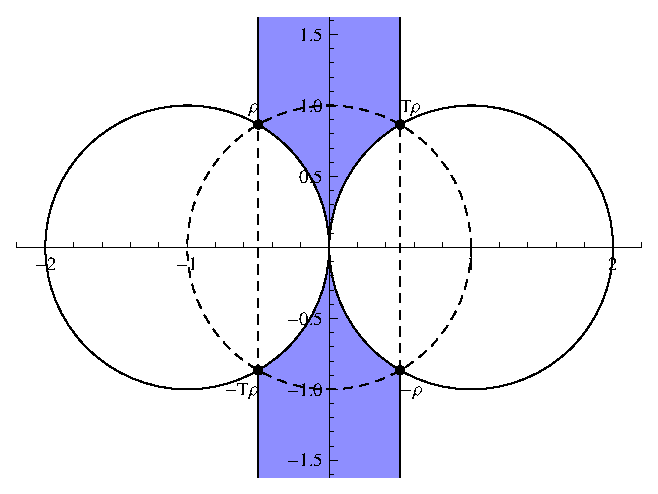
\includegraphics[width=0.8\textwidth]{figures/minimal-region}
\caption{The region of numbers $z \in \EC$, where $\Re{z}$ and $\Re{\reci{z}}$ are both contained in the interval $\left[-\half{1},\half{1}\right]$ is obtained by taking the strip $\Re{z} \in \left[-\half{1},\half{1}\right]$ and cutting out two disks of unit radius centered about the real points $\pm 1$. The arising vertices are labeled. As usual, $T$ is the transformation $z \mapsto -\reci{z}$ and $\rho = \exp(2 \pi \ii / 3)$ is a third root of unity.}
\label{fig_MinimalRegion}
\end{figure}

\begin{figure}
\centering
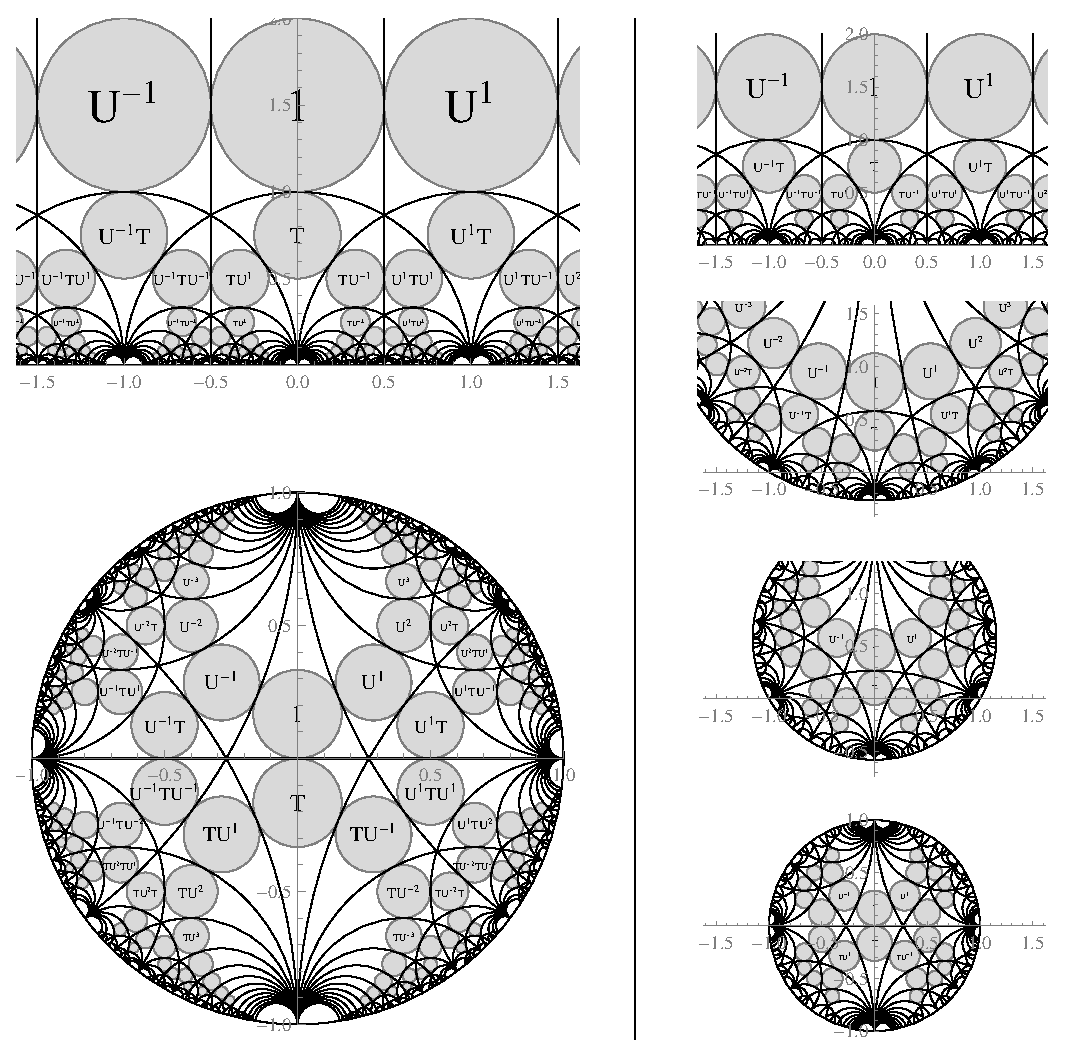
\includegraphics[width=\textwidth]{figures/modular-tiling-1}
\caption{The tessellation of the upper halfplane.}
\label{fig_ModularTiling}
\end{figure}

\begin{figure}
\centering
\includegraphics[width=0.8\textwidth]{figures/modular-tiling-exp-fan}
\caption{The tessellation under the transformation $z \mapsto \exp(2 \pi \ii z)$.}
\label{fig_ModularTilingExpFan}
\end{figure}

\begin{figure}
\centering
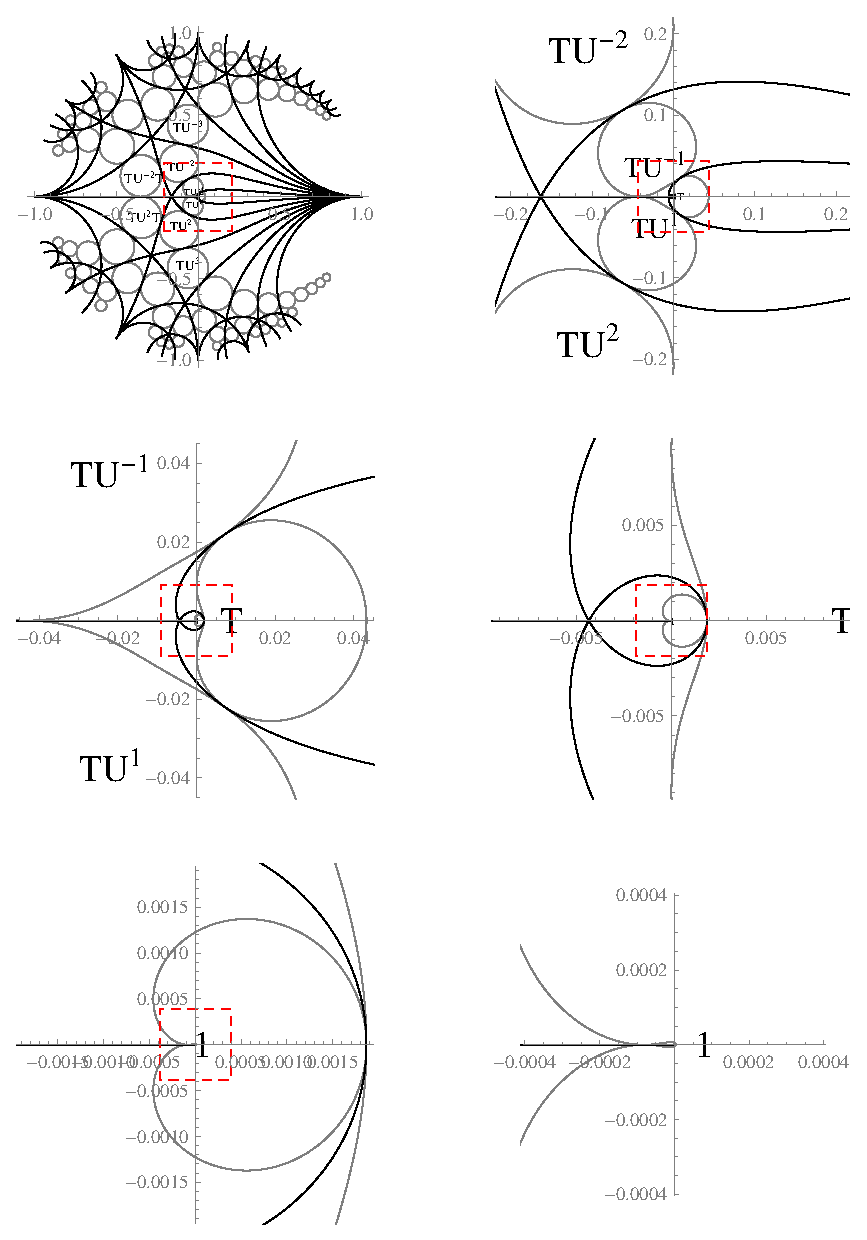
\includegraphics[width=0.8\textwidth]{figures/modular-tiling-exp-zoom}
\caption{The image of the modular tiling under the map $z \mapsto \exp(2 \pi \ii z)$ in the neighborhood of $\infty$.}
\label{fig_ModularTilingExpZoom}
\end{figure}


% --------------------------------------------- Subsection: Hyperbolic geometry
\subsection{Hyperbolic geometry}

\todo{11}{Connection to hyperbolic geometry (disk/halplane model)}


% ------------------------------- Subsection: Ford circles, continued fractions
\subsection{Ford circles and continued fractions}

For an arbitrary modular transformation $A$, a representation as product of shifts $U^j: z \mapsto z+j$ and inversions $T: z \mapsto -\reci{z}$ can be found by the algorithm described in Corollary \ref{cor_ModGrpTUAlg}. By writing out this product, for example in the case, when $n=2$, we have
\begin{equation*}
A = U^{e_0}T U^{e_1}T U^{e_2}T U^k,
\end{equation*}
or more explicitly
\begin{equation}
\label{eqn_ALongConFrac}
A(z) = e_0 - \reci{e_1 - \reci{e_2 - \reci{k + z}}}.
\end{equation}
\index{Continued fraction}
Here, a close relation between modular transformations and continued fractions immediately gets apparent. In this section, we will investigate this relation somewhat deeper. 
First, we will use Pringsheim's more space-saving notation for continued fractions, namely
\begin{equation}
\label{eqn_ConFracNotation}
b_0 + \frac{a_1}{b_1 + \frac{a_2}{b_2 + \frac{a_3}{b_3 + \dots}}} =: 
b_0 + \cfr{a_1}{b_1} + \cfr{a_2}{b_2} + \cfr{a_2}{b_3} + \dots
\end{equation}
In the case when all $a_j = 1$, we adhere to the standard sequence notation for continued fractions:
\begin{equation*}
b_0 + \reci{b_1 + \reci{b_2 + \dots}} =: [b_0,b_1,b_2,\dots].
\end{equation*}
We can now reformulate Corollary \ref{cor_ModGrpTUAlg} in order to construct a continued fraction representation of any given modular transformation.

\begin{corollary}
An arbitrary modular transformation $A(z) = \moebius{a}{b}{c}{d}{z}$ can be written as continued fraction
\begin{equation}
\label{eqn_ModTransConFrac}
A(z) = [q_0,q_1,\dots,q_n,(-1)^{n+1}(k+z)]
\end{equation}
where the integers $n$, $q_0,q_1,\dots,q_n$ and $k$ are determined by the algorithm described in Corollary \ref{cor_ModGrpTUAlg}.
\end{corollary}
\begin{proof}
By using the continued fraction representation of $A$ given in (\ref{eqn_ALongConFrac}) and by applying the definition $e_j$ := $(-1)^j q_j$ we have
\begin{IEEEeqnarray}{rCcCcCcCcCcCc}
A(z) &=& e_0 &+& \cfr{-1}{e_1} 
          &+& \cfr{-1}{e_2} 
          &+& \dots 
          &+& \cfr{-1}{e_n} 
          &+& \cfr{-1}{k + z} \nonumber \\
  &=& q_0 &+& \cfr{-1}{-q_1} 
          &+& \cfr{-1}{q_2} 
          &+& \dots 
          &+& \cfr{-1}{(-1)^n q_n} 
          &+& \cfr{-1}{k + z}. \label{eqn_ModTransConFracInterim}
\end{IEEEeqnarray}
Now, for every odd $j \le n$, we can rewrite 
\begin{equation*}
\cfr{-1}{-q_j} + \cfr{-1}{\dots} \quad \text{to} \quad \cfr{1}{q_j} + \cfr{1}{\dots}.
\end{equation*}
Thus, if $n$ is odd, every numerator $-1$ in (\ref{eqn_ModTransConFracInterim}) can be turned into $+1$. In the other case, when $n$ is even, only one negative numerator at the end, $\frac{-1}{k+z}$, remains, but this can easily be rewritten to $\frac{1}{-(k+z)}$. Taking both cases together, we obtain (\ref{eqn_ModTransConFrac}).
\end{proof}

\todo{19}{The modular group and ford circles}


